%%% MORITZ 2.5' %%%

\section{Doppelresonanz}
\subsection{Grundlagen: Optisches Pumpen}


\begin{frame}
\frametitle{Zeeman-Aufspaltung der Hyperfeinstruktur}

\setbeamerfont{myfont}{size*=80}
\usebeamerfont{myfont}

\begin{figure}
    \centering
    \def\svgwidth{\textwidth}
    \input{../img/termschema_rot.pdf_tex}
    \caption{Zeeman-Aufspaltung der Hyperfeinstruktur von \rb{85} und \rb{87}.}
\end{figure}

\end{frame}



\begin{frame}
\frametitle{Optisches Pumpen}

\setbeamerfont{myfont}{size*=80}
\usebeamerfont{myfont}
\begin{figure}
   \centering
    \def\svgwidth{\textwidth}
    \input{../img/optPumpen0.pdf_tex}
    \caption{Zeeman-Pumpen von \rb{87} mit \textsigma$^+$-Licht.}
\end{figure}

\end{frame}




\begin{frame}[noframenumbering]
\frametitle{Optisches Pumpen}

\setbeamerfont{myfont}{size*=80}
\usebeamerfont{myfont}
\begin{figure}
   \centering
    \def\svgwidth{\textwidth}
    \input{../img/optPumpen.pdf_tex}
    \caption{Zeeman-Pumpen von \rb{85} mit \textsigma$^+$-Licht.}
\end{figure}

\end{frame}


\subsection{Aufbau}
\begin{frame}
\frametitle{Aufbau: Doppelresonanz}

\setbeamerfont{myfont}{size*=80}
\usebeamerfont{myfont}
\begin{figure}
    \centering
    \def\svgwidth{\textwidth}
    \input{../img/aufbauDR.pdf_tex}
    \caption{Aufbau zur Messung der Doppelresonanz.}
\end{figure}
\usebeamerfont{standard}

\begin{itemize}
  \item \textbf{\textlambda/4-Plättchen:} Erzeugung von zirkular polarisiertem Licht
  \item \textbf{Spule 1:} Einstellbarer Gleichstrom
  \item \textbf{Spule 2:} Sinusförmiger Strom
  \item \textbf{Spule 4:} Kompensation von vertikalem Erdmagnetfeld
  \item \textbf{RF-Sender:} Einstrahlung von elmag. Wechselfeld in die Messzelle
\end{itemize}

\end{frame}

\subsection{Messung}

\begin{frame}
\frametitle{Messung: Doppelresonanz}
\begin{figure}
    \begin{center}
        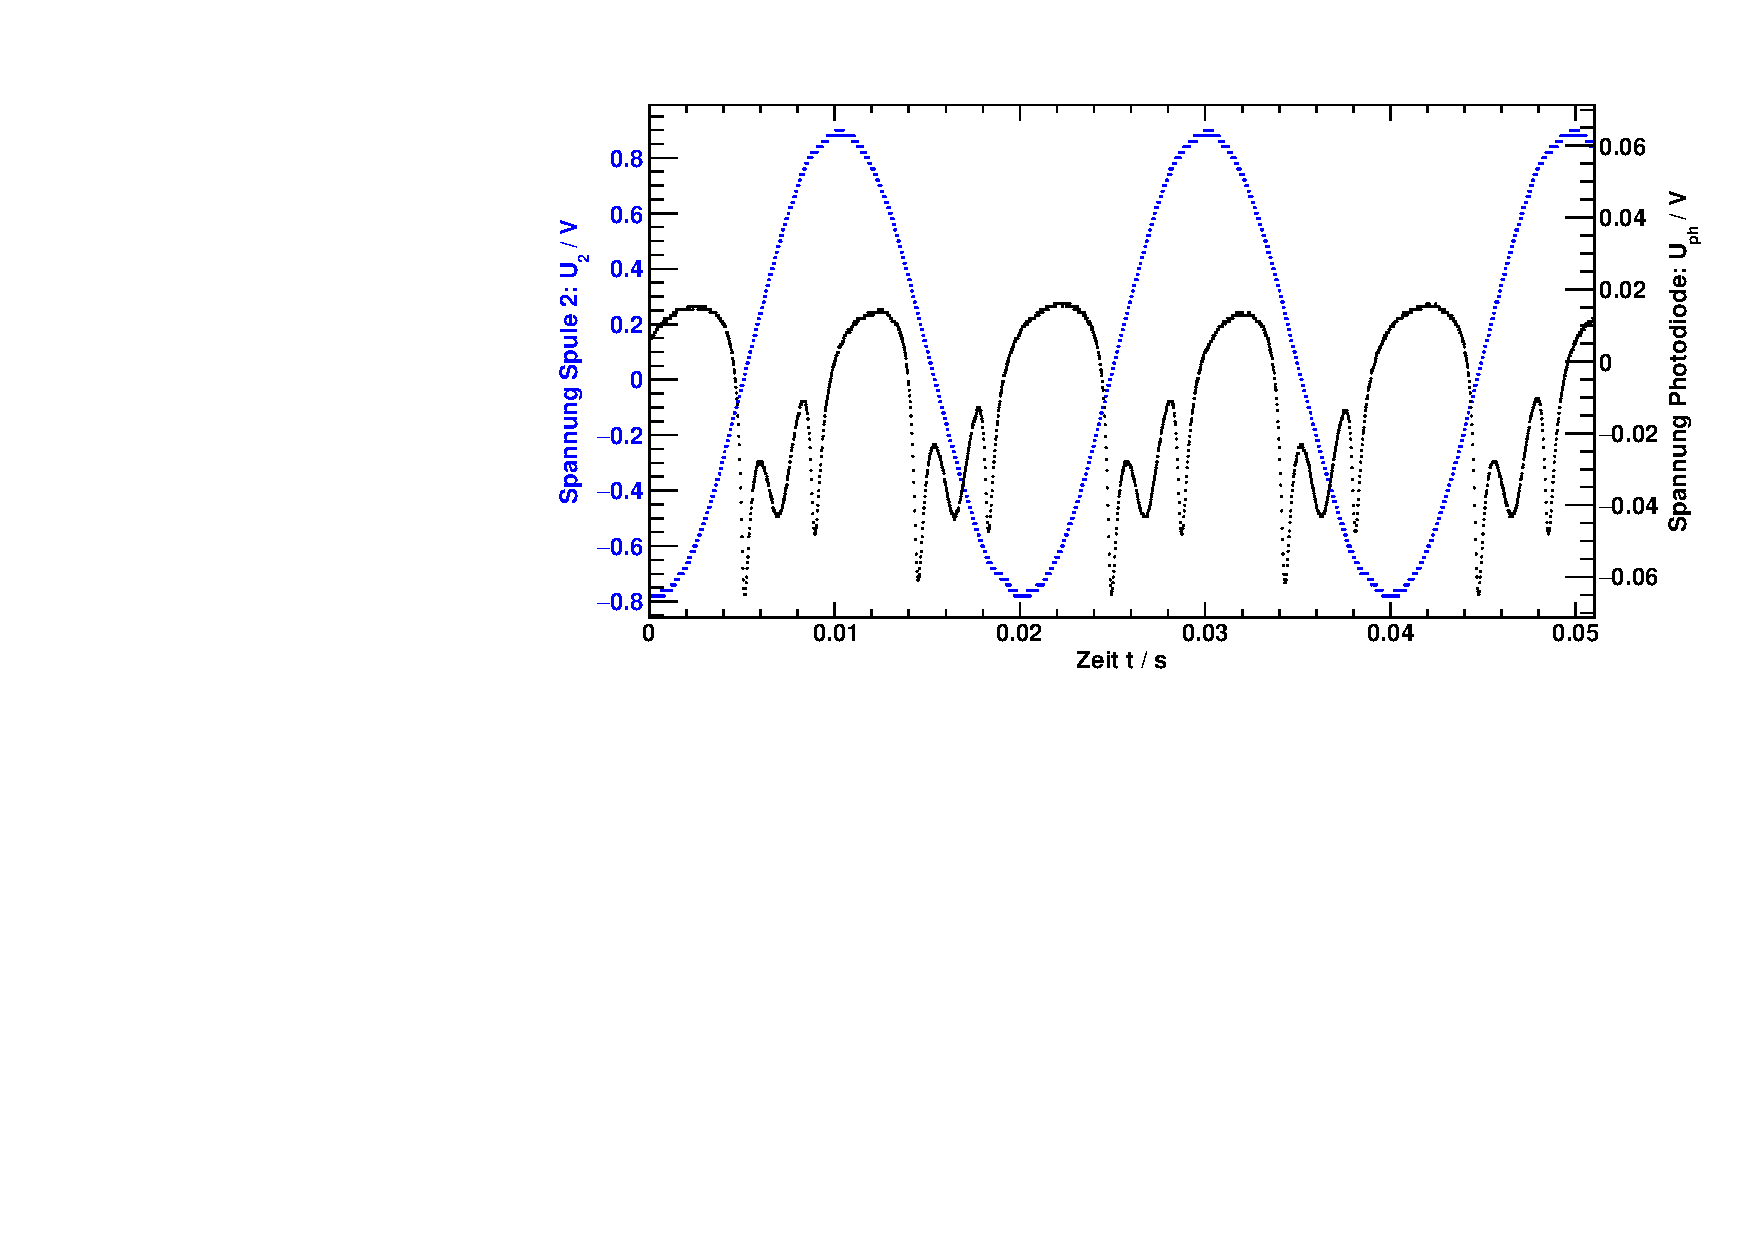
\includegraphics[width=\textwidth]{../img/06.pdf}
        \caption{Doppelresonanz mit Störsignal.}
        \label{img:dehmeltrf}
    \end{center}
\end{figure}
\end{frame}


\begin{frame}
\frametitle{Messung: Doppelresonanz}
\begin{figure}
    \begin{center}
        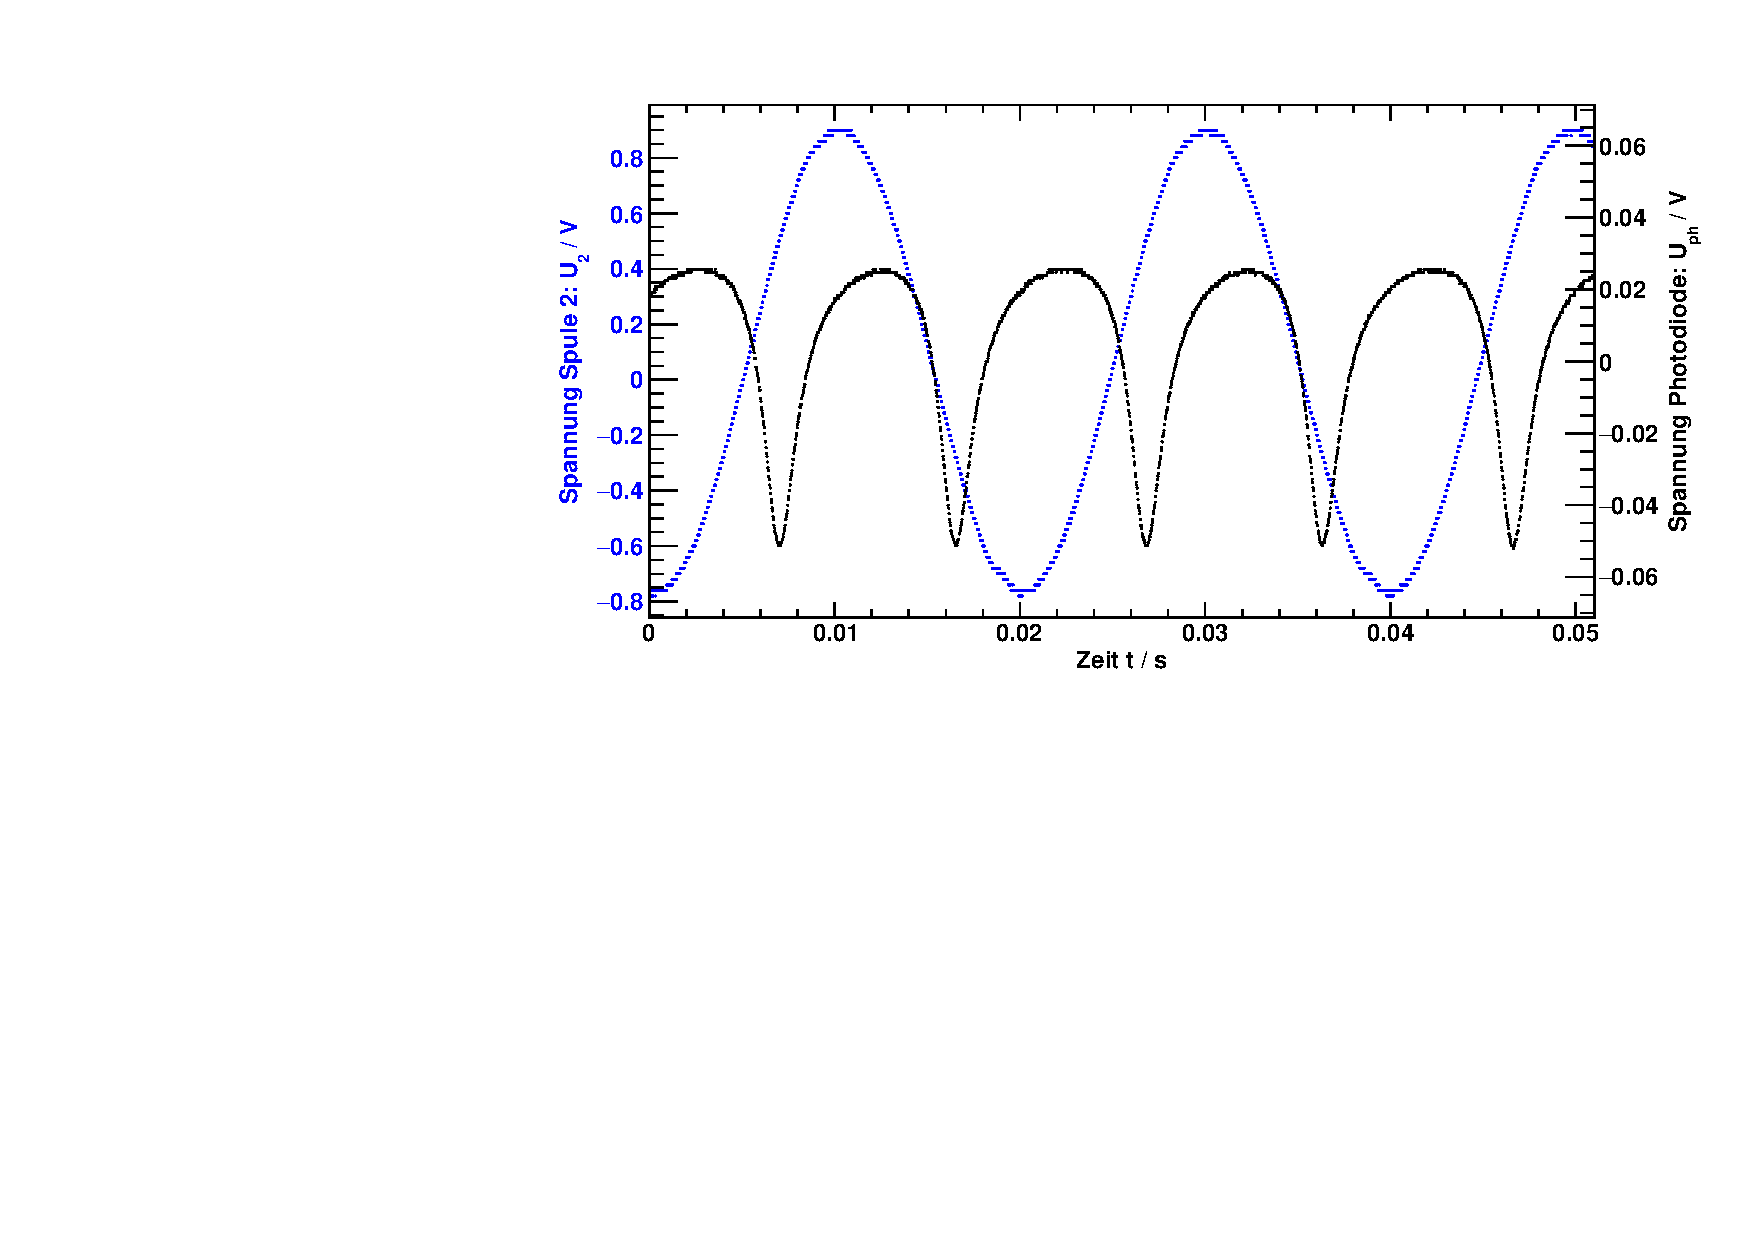
\includegraphics[width=\textwidth]{../img/07.pdf}
        \caption{Störsignal bei Messung ohne RF-Signal.}
        \label{img:dehmelt}
    \end{center}
\end{figure}
\end{frame}


\begin{frame}
\frametitle{Messung: Doppelresonanz}
\begin{figure}
    \begin{center}
        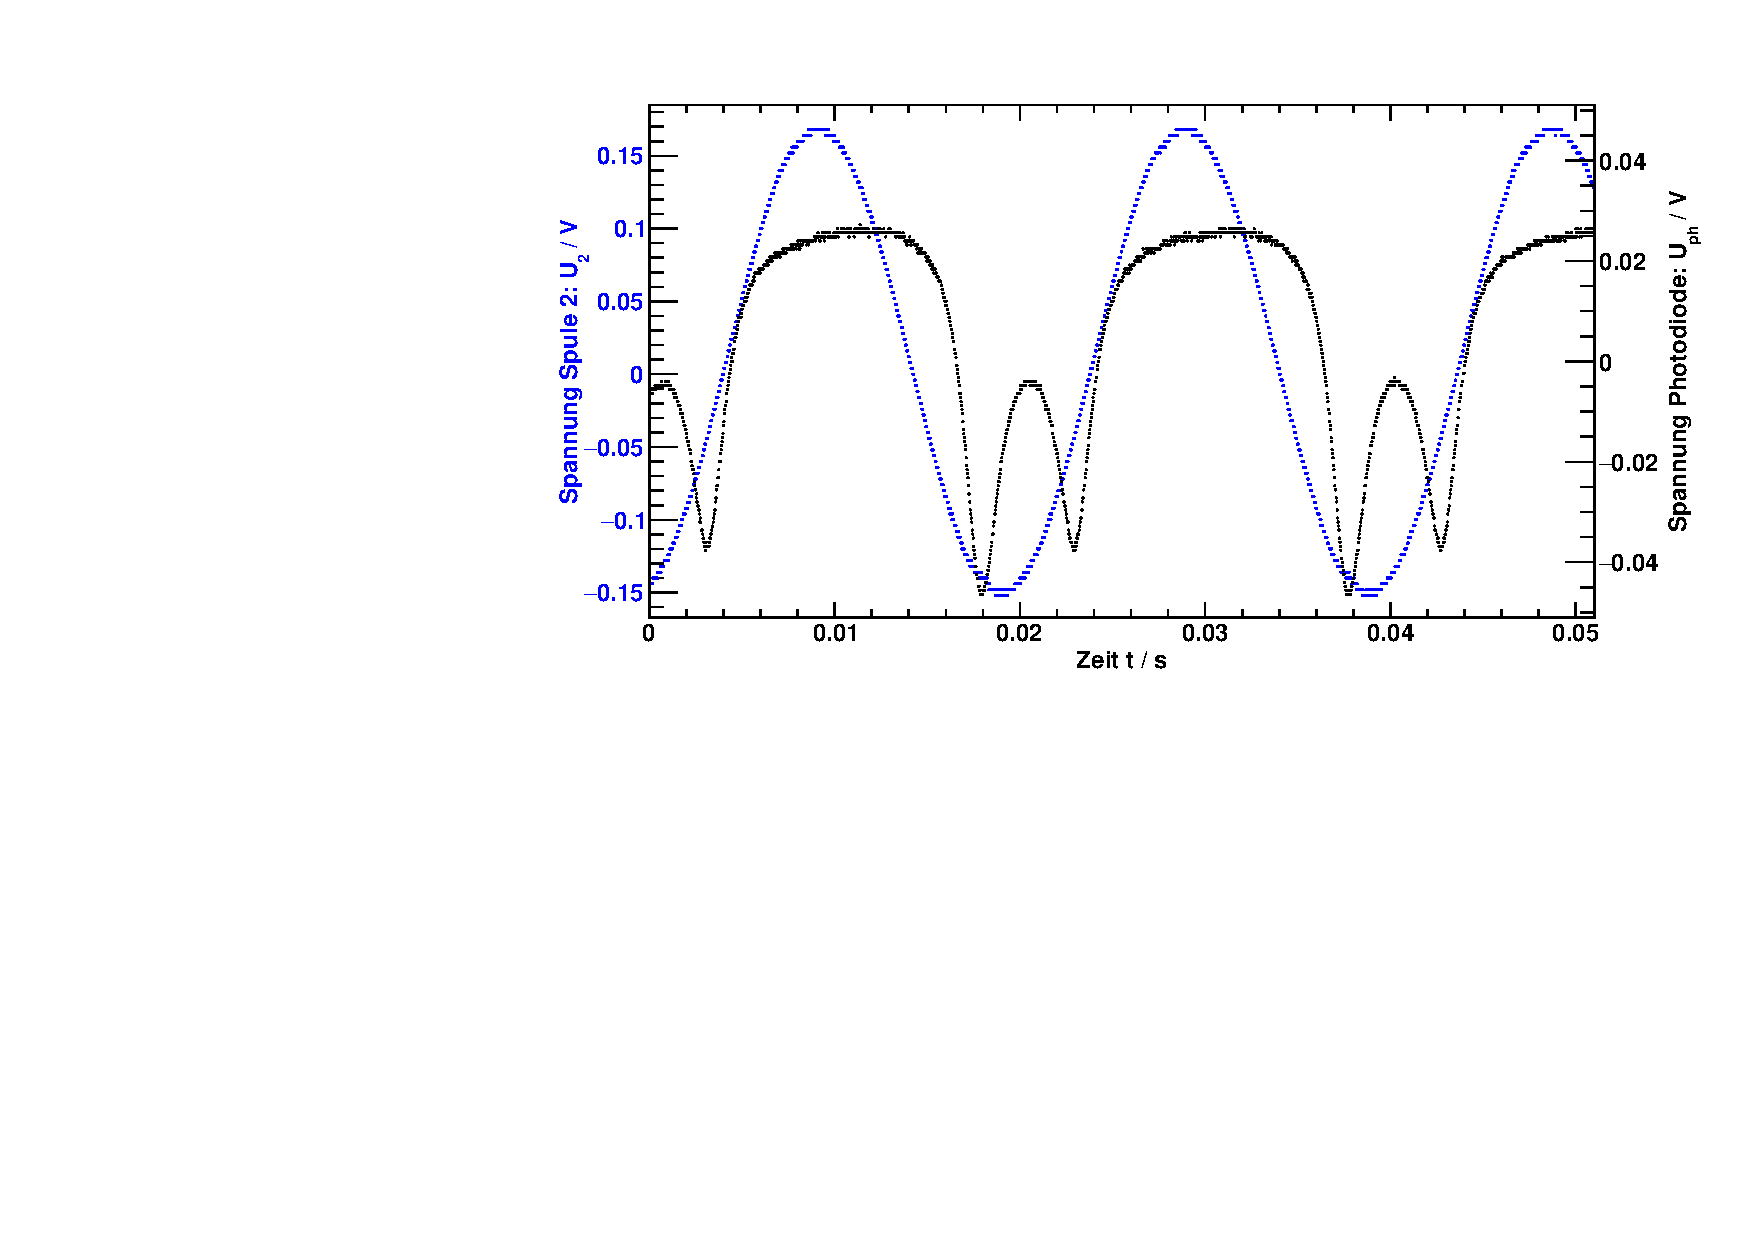
\includegraphics[width=\textwidth]{../img/11.pdf}
        \caption{Doppelresonanz-Absorptionssignal bei kleiner Magnetfeldmodulation:
        Falsche Einstellung des Gleichstroms in Spule~1,
        die Absorptionen sind nicht äquidistant.}
        \label{img:rfwrong}
    \end{center}
\end{figure}
\end{frame}


\begin{frame}
\frametitle{Messung: Doppelresonanz}
\begin{figure}
    \begin{center}
        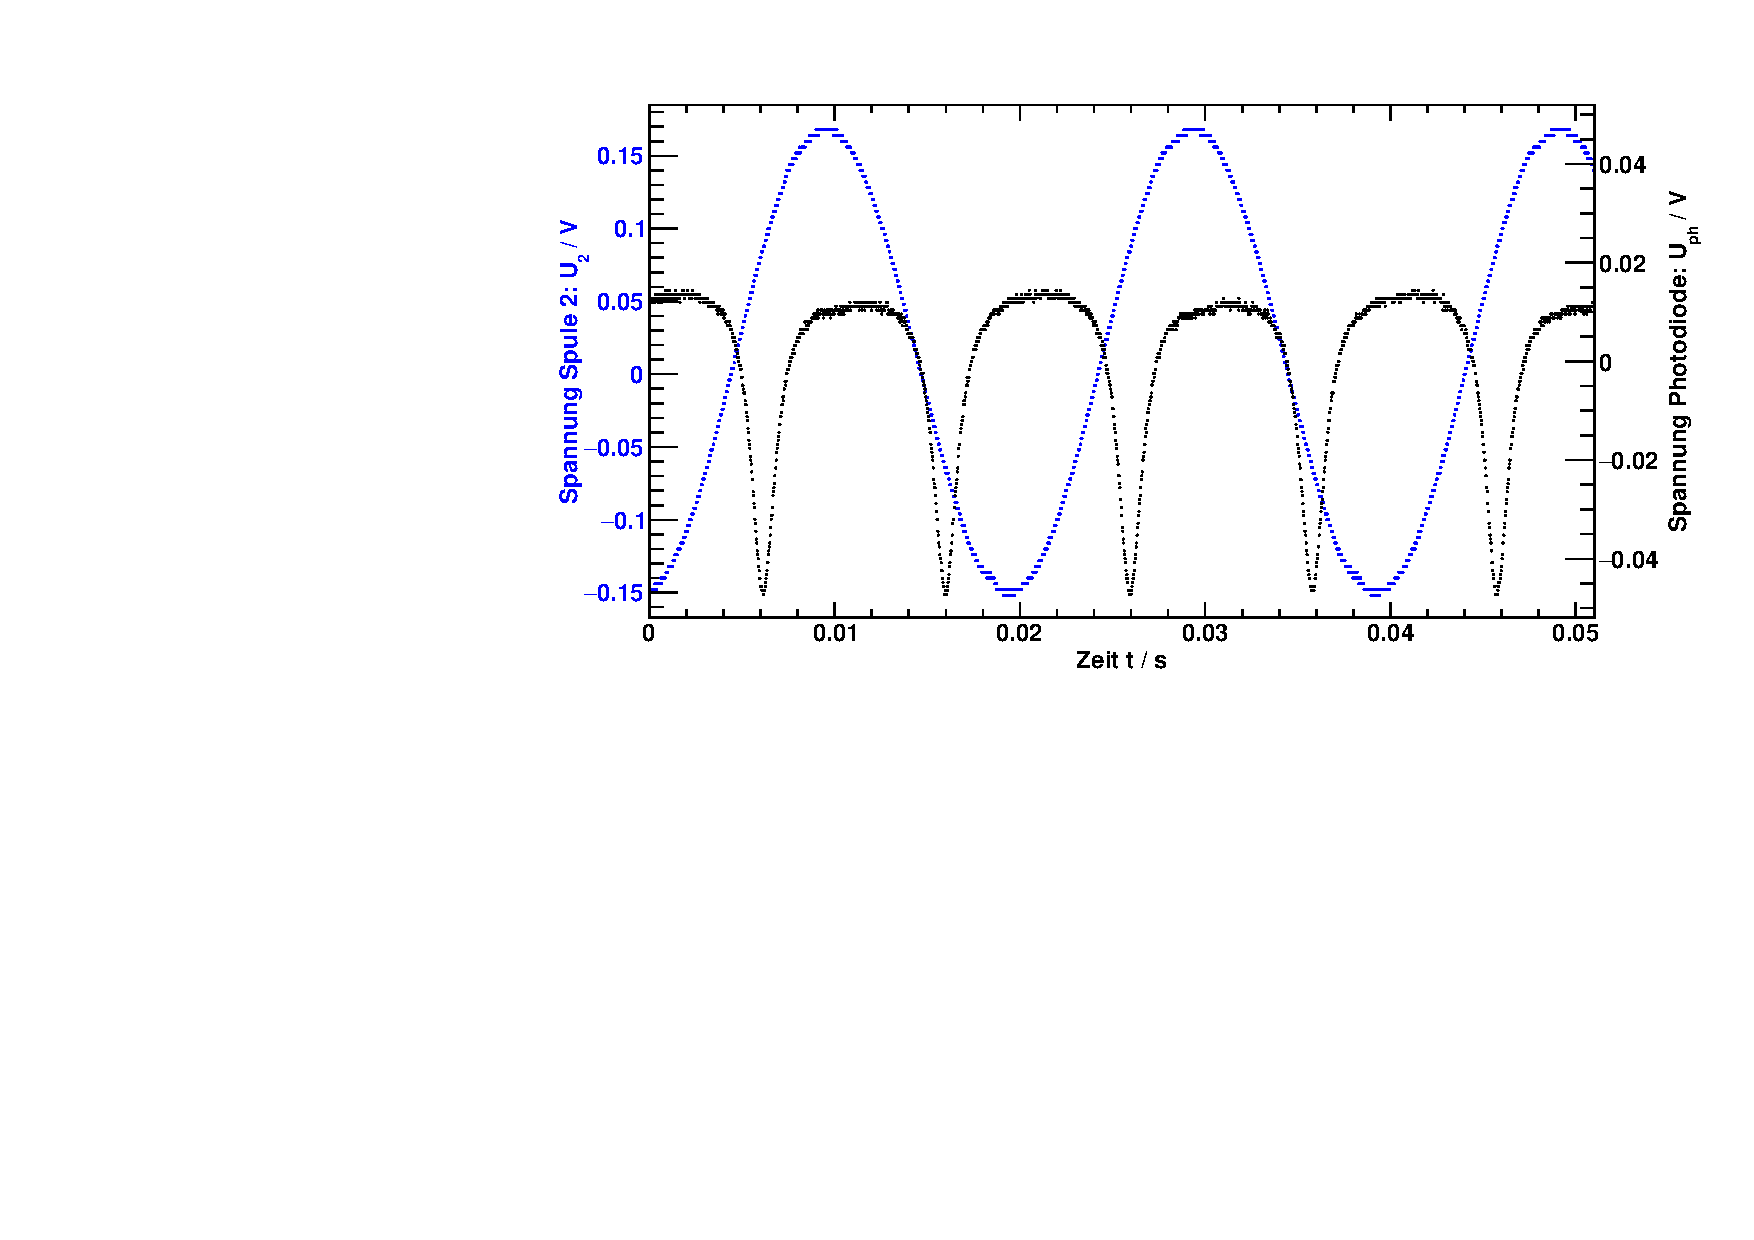
\includegraphics[width=\textwidth]{../img/08.pdf}
        \caption{Doppelresonanz-Absorptionssignal bei kleiner Magnetfeldmodulation:
        Korrekte Einstellung des Gleichstroms in Spule~1,
        die Absorptionen sind daher äquidistant.}
        \label{img:rfcorrect}
    \end{center}
\end{figure}
\end{frame}


%%% BEN 2.5' %%%

\subsection{Auswertung}
\begin{frame}
\frametitle{Auswertung: Erdmagnetfeld und Kernspin}
\begin{itemize}[<+->]
    \item Umrechnung Spulenstrom $\leftrightarrow$ Magnetfeld
    \item Horizontales Magnetfeld
    \begin{equation*}
        B_\text{hor} = \frac{1}{2} \abs{B_1 - B_1'}
    \end{equation*}
    \item Vertikales Magnetfeld
    \begin{equation*}
        B_\text{ver} = B_4
    \end{equation*}
    \item Magnetfeld zur Berechnung des Kernspins $I$
    \begin{equation*}
        \begin{split}
            B_I &= \frac{B_1 + B_1'}{2} \\
            \Rightarrow I &= \frac{\mu_B \cdot B_I}{h \cdot \nu} - \frac{1}{2}
        \end{split}
    \end{equation*}
\end{itemize}
\end{frame}


\begin{frame}
\frametitle{Ergebnisse: Erdmagnetfeld und Kernspin}
\begin{table}
    \caption{Berechnete horizontale Komponenten des Erdmagnetfeldes und Kernspin von Rubidium für das Doppelresonanzexperiment bei verschiedenen Lasterströmen $I_\text{L}$ und RF-Sender-Frequenzen $\nu$.}
    \begin{center}
        \begin{tabular}{|c|c|c|c|c|}
            \hline
            $I_\text{L}$ / mA & $\nu$ / kHz & $B_\text{hor}$ / \textmu T & $I$ \\ \hline
            62.9 & 493.98 & $12.4 \pm 1.1$ & $2.50 \pm 0.03$ \\ \hline
            62.9 & 899.41 & $12.8 \pm 2.3$ & $2.53 \pm 0.04$ \\ \hline
            63.2 & 493.77 & $12.0 \pm 1.1$ & $1.52 \pm 0.03$ \\ \hline
            63.2 & 899.67 & $12.4 \pm 1.1$ & $1.53 \pm 0.02$ \\ \hhline{|==|=|=|}
            \multicolumn{2}{|c|}{gew. Mittel \rb{85}} & \multirow{2}{*}{$12.3 \pm 0.6$} & $2.51 \pm 0.02$ \\ \cline{1-2} \cline{4-4}
            \multicolumn{2}{|c|}{gew. Mittel \rb{87}} & & $1.527 \pm 0.016$ \\ \hline
            \multicolumn{2}{|c|}{Lit./theo. Wert \rb{85}} & \multirow{2}{*}{$20.9$} & 2.5 \\ \cline{1-2} \cline{4-4}
            \multicolumn{2}{|c|}{Lit./theo. Wert \rb{87}} & & 1.5 \\ \hline
        \end{tabular}
    \end{center}
\end{table}
\begin{equation*}
    \begin{split}
        & B_\text{ver} = (40.94 \pm 1.43)\,\text{\textmu T} \\
        & B_\text{ver}^{\text{Lit.}} = 42.9\,\text{\textmu T}
    \end{split}
\end{equation*}
\end{frame}